\documentclass[11pt,a4paper]{article}

% ------------------------------------------------------------------
% Paquetes
% ------------------------------------------------------------------
\usepackage[utf8]{inputenc}
\usepackage[T1]{fontenc}
\usepackage[spanish,es-tabla,es-nodecimaldot]{babel}
\usepackage{lmodern}
\usepackage[margin=2.5cm]{geometry}
\usepackage{amsmath,amssymb}
\usepackage{graphicx}
\usepackage{booktabs}
\usepackage{tabularx}
\usepackage{multirow}
\usepackage{float}
\usepackage{caption}
\usepackage{xcolor}
\usepackage{algorithm}
\usepackage{algpseudocode}
\usepackage{enumitem}
\usepackage[hidelinks]{hyperref}
\usepackage[numbers,sort&compress]{natbib}

\graphicspath{{figuras/}}
\captionsetup{font=small,labelfont=bf}
\floatname{algorithm}{Algoritmo}
\renewcommand{\algorithmicrequire}{\textbf{Entrada:}}
\renewcommand{\algorithmicensure}{\textbf{Salida:}}
\setlength{\parskip}{0.4em}

% ------------------------------------------------------------------
\title{\textbf{Problema de Cubrimiento de Conjuntos (SET COVER):\\
Solución exacta mediante programación lineal entera\\
y un algoritmo genético}}
\author{Integrante 1 \and Integrante 2\\[2pt]
\small Proyecto de clase -- Optimización}
\date{Noviembre de 2026}

\begin{document}
\maketitle

\begin{abstract}
Este trabajo aborda el problema de cubrimiento de conjuntos (\emph{Set Covering Problem}, SCP) con costos,
un problema clásico de optimización combinatoria NP-difícil. Se formula el modelo de programación lineal
entera binaria, se resuelve de forma exacta con PuLP y el solver CBC, y se diseña e implementa un
algoritmo genético (AG) basado en Beasley y Chu, con codificación binaria, cruce por fusión, mutación de
tasa variable y un operador de reparación especializado. Ambos métodos se comparan sobre las 18
instancias de los conjuntos 4 y 5 de la OR-Library y sobre instancias aleatorias de tamaño creciente. En
las instancias de la OR-Library el método exacto obtuvo y probó el óptimo en menos de 0,2~s, mientras que
el AG alcanzó el óptimo en 15 de las 18 instancias (al menos en una de sus 10 corridas) con un gap
promedio de 0,58\% y un tiempo medio de 3,3~s. En instancias grandes la situación se invierte: el
tiempo del solver crece de forma exponencial y, con un límite de 180~s, el AG encontró soluciones iguales
o mejores que la mejor solución entera de CBC en una fracción del tiempo. Todo el desarrollo se acompaña
de una interfaz visual que permite ejecutar y comparar ambos métodos.
\end{abstract}

% ==================================================================
\section{Descripción del problema}
% ==================================================================
El problema de cubrimiento de conjuntos consiste en lo siguiente: se tiene un conjunto de
$m$ elementos (filas) y una colección de $n$ subconjuntos (columnas), cada uno con un costo
$c_j>0$. Cada subconjunto cubre a algunos elementos. El objetivo es seleccionar un grupo de
subconjuntos de costo total mínimo tal que \emph{cada elemento quede cubierto al menos una
vez}~\citep{caprara2000,beasley1996ga}.

El SCP modela numerosas aplicaciones reales: la asignación de tripulaciones en aerolíneas y
ferrocarriles, la localización de servicios de emergencia (ubicar el menor número de
estaciones para que toda la zona quede atendida), el diseño de redes y la selección de casos de
prueba, entre otras~\citep{caprara2000}. Su versión de decisión está entre los 21 problemas
NP-completos de Karp~\citep{karp1972,garey1979}, por lo que no se conoce un algoritmo que lo
resuelva en tiempo polinomial. Esto motiva la comparación de este proyecto: un método
\emph{exacto}, que garantiza el óptimo pero cuyo tiempo puede crecer de forma exponencial, frente a
una \emph{metaheurística}, que no garantiza el óptimo pero suele encontrar buenas soluciones
rápidamente.

\paragraph{Objetivos.} (i) Formular el modelo matemático del SCP; (ii) resolverlo de forma exacta
con un solver de optimización; (iii) diseñar e implementar un algoritmo genético; (iv) comparar
ambos enfoques en calidad de la solución, tiempo de cómputo y comportamiento; y (v) construir una
interfaz visual para ejecutar e interpretar los resultados.

% ==================================================================
\section{Formulación matemática}
% ==================================================================
\subsection*{Conjuntos e índices}
\begin{itemize}[nosep]
  \item $I=\{1,\dots,m\}$: conjunto de filas (elementos que deben cubrirse), índice $i$.
  \item $J=\{1,\dots,n\}$: conjunto de columnas (subconjuntos disponibles), índice $j$.
\end{itemize}

\subsection*{Parámetros}
\begin{itemize}[nosep]
  \item $c_j$: costo de seleccionar la columna $j$, $\forall j\in J$.
  \item $a_{ij}=1$ si la columna $j$ cubre la fila $i$, y $a_{ij}=0$ en otro caso. La matriz
  $A=(a_{ij})$ de tamaño $m\times n$ es la \emph{matriz de cobertura}.
\end{itemize}

\subsection*{Variable de decisión}
\[
x_j=\begin{cases}1,& \text{si se selecciona la columna } j,\\ 0,& \text{en otro caso,}\end{cases}
\qquad \forall j\in J.
\]

\subsection*{Modelo}
\begin{align}
\min\; & Z=\sum_{j=1}^{n} c_j\,x_j \label{eq:fo}\\
\text{s.a.}\; & \sum_{j=1}^{n} a_{ij}\,x_j \;\ge\; 1, && \forall i\in I \label{eq:cob}\\
& x_j\in\{0,1\}, && \forall j\in J \label{eq:dom}
\end{align}

\paragraph{Interpretación.} La función objetivo~\eqref{eq:fo} suma el costo de todas las columnas
seleccionadas; se busca que sea mínima. La restricción~\eqref{eq:cob} es la restricción de
\emph{cobertura}: para cada fila $i$, la suma cuenta cuántas columnas seleccionadas la cubren, y
exigir que sea al menos 1 garantiza que ningún elemento quede sin cubrir. Hay una restricción por
fila, es decir, $m$ restricciones. Finalmente,~\eqref{eq:dom} indica que cada subconjunto se toma
completo o no se toma, lo que da $n$ variables binarias. El modelo es un problema de
programación lineal entera binaria (PLEB) con $n$ variables y $m$ restricciones.

\paragraph{Ejemplo.} Con $m=4$ elementos y las columnas $S_1=\{1,2\}$ ($c_1=3$),
$S_2=\{2,3\}$ ($c_2=2$), $S_3=\{3,4\}$ ($c_3=3$) y $S_4=\{1,4\}$ ($c_4=2$), la solución
$x_2=x_4=1$ cubre los cuatro elementos con costo 4, que es el mínimo: cualquier otra pareja cuesta
al menos 5, y ninguna columna sola cubre todo.

% ==================================================================
\section{Metodología de solución exacta}
% ==================================================================
El modelo~\eqref{eq:fo}--\eqref{eq:dom} se resuelve con el solver de código abierto CBC
(\emph{COIN-OR Branch and Cut})~\citep{forrest2005cbc}, a través de la librería PuLP de
Python~\citep{mitchell2011pulp}. CBC aplica el método de ramificación y acotamiento
(\emph{branch-and-bound})~\citep{landdoig1960}: resuelve la relajación lineal (cambiando
$x_j\in\{0,1\}$ por $0\le x_j\le 1$), cuyo valor es una cota inferior del óptimo, y si la solución
tiene variables fraccionarias divide el problema en dos subproblemas ($x_j=0$ y $x_j=1$). Además
agrega planos de corte, desigualdades válidas que eliminan soluciones fraccionarias sin eliminar
soluciones enteras, y usa heurísticas para encontrar soluciones enteras
tempranamente~\citep{wolsey2020}. Un nodo se descarta cuando su cota es peor que la mejor solución
entera conocida. Cuando la cota inferior global y la mejor solución coinciden, el solver
\emph{prueba} que la solución es óptima.

\paragraph{Implementación.} El archivo \texttt{src/exacto.py} construye el modelo así:
\begin{enumerate}[nosep]
  \item Crea las $n$ variables \texttt{LpVariable(..., cat="Binary")}.
  \item Define el objetivo \texttt{lpDot(c, x)}.
  \item Agrega una restricción \texttt{lpSum(x[j] for j in cols\_de\_fila[i]) >= 1} por cada fila.
  Solo se suman las columnas que cubren la fila, lo que equivale a usar los $a_{ij}=1$ y aprovecha
  que la matriz es dispersa (densidad de 2\%).
  \item Resuelve con \texttt{PULP\_CBC\_CMD} con un límite de tiempo configurable.
\end{enumerate}
Se reportan el costo, las columnas seleccionadas, el tiempo de construcción y de solución, y el
estado: \emph{óptimo probado} o \emph{solución factible al límite de tiempo}. El método es
determinista, por lo que los resultados son reproducibles.

% ==================================================================
\section{Diseño del algoritmo genético}
% ==================================================================
Los algoritmos genéticos imitan la evolución natural: una población de soluciones candidatas
evoluciona mediante selección, cruce y mutación, favoreciendo a los individuos más
aptos~\citep{holland1975,goldberg1989,eiben2015}. El diseño sigue el AG propuesto por
\citet{beasley1996ga} para el SCP con costos, que introdujo el cruce por fusión, la mutación de
tasa variable y un operador de reparación específico para el problema.

\subsection{Codificación (cromosoma)}
Cada individuo es un vector binario de longitud $n$, $\mathbf{x}=(x_1,\dots,x_n)$. El gen $j$
vale 1 si la columna $j$ está en la solución. Esta codificación coincide con la variable de decisión del
modelo exacto, lo que facilita comparar las soluciones. Por ejemplo, para $n=6$, el
cromosoma $(0,1,0,0,1,1)$ representa la selección de las columnas 2, 5 y 6.

\subsection{Función de aptitud}
La aptitud de un individuo es su costo, $f(\mathbf{x})=\sum_j c_j x_j$, y \emph{se minimiza}: un
individuo es más apto cuanto menor es su costo. No se necesita penalizar la infactibilidad porque
el operador de reparación (sección~\ref{sec:rep}) garantiza que \emph{todos} los individuos cubran
todas las filas.

\subsection{Operador de reparación}\label{sec:rep}
Después del cruce y la mutación un hijo puede dejar filas sin cubrir o tener columnas redundantes.
El operador de reparación (Algoritmo~\ref{alg:rep}) actúa en dos pasos:
\begin{enumerate}[nosep]
  \item \textbf{Factibilidad.} Para cada fila sin cubrir agrega la columna que la cubre con menor
  costo por fila nueva cubierta, es decir, que minimiza $c_j / |\text{filas descubiertas que cubre } j|$.
  Es el mismo criterio de la heurística voraz de \citet{chvatal1979}.
  \item \textbf{Eliminación de redundancia.} Recorre las columnas seleccionadas de mayor a menor
  costo y elimina cada una cuyas filas siguen cubiertas por otras columnas.
\end{enumerate}
El segundo paso convierte cada solución en un cubrimiento \emph{mínimo} (ninguna columna sobra),
lo que mejora mucho la calidad de los individuos.

\begin{algorithm}[H]
\caption{Operador de reparación}\label{alg:rep}
\begin{algorithmic}[1]
\Require individuo $\mathbf{x}$; cobertura $w_i=\sum_j a_{ij}x_j$ de cada fila
\For{cada fila $i$ con $w_i=0$}
  \State $j^\ast \gets \arg\min_{j:\,a_{ij}=1} \; c_j \,/\, |\{k: w_k=0,\ a_{kj}=1\}|$
  \State $x_{j^\ast}\gets 1$; actualizar $w$
\EndFor
\For{cada $j$ con $x_j=1$, en orden decreciente de $c_j$}
  \If{$w_k\ge 2$ para toda fila $k$ con $a_{kj}=1$}
     \State $x_j\gets 0$; actualizar $w$ \Comment{la columna $j$ es redundante}
  \EndIf
\EndFor
\Ensure $\mathbf{x}$ factible y sin columnas redundantes
\end{algorithmic}
\end{algorithm}

\subsection{Inicialización de la población}
Cada uno de los $N$ individuos iniciales se construye así: para cada fila $i$ se elige \emph{al azar} una
de las columnas que la cubren, y luego se aplica el paso de eliminación de redundancia. El
resultado es una población factible y diversa, ya que no depende de ninguna heurística voraz.

\subsection{Selección}
Se usa \textbf{torneo binario}: se toman dos individuos al azar y gana el de menor costo. Se
realizan dos torneos independientes para obtener los dos padres (distintos). El torneo da más
oportunidad a los mejores individuos sin eliminar a los demás, lo que mantiene diversidad, y no
depende de la escala de la aptitud~\citep{goldberg1989}.

\subsection{Cruce por fusión}
Dados los padres $P_1$ y $P_2$ con aptitudes $f_1$ y $f_2$, el hijo $H$ se construye gen por gen:
\[
H_j=\begin{cases}
P_{1j}, & \text{si } P_{1j}=P_{2j},\\
P_{1j} \text{ con probabilidad } \dfrac{f_2}{f_1+f_2}, \text{ o } P_{2j} \text{ en otro caso}, & \text{si } P_{1j}\neq P_{2j}.
\end{cases}
\]
Los genes en que coinciden ambos padres se heredan directamente. En los genes en que difieren, el
padre más barato tiene mayor probabilidad de transmitir su gen~\citep{beasley1996ga}. Es un cruce
uniforme sesgado por la aptitud.

\subsection{Mutación de tasa variable}
Se invierten $k(t)$ bits elegidos al azar, donde $t$ es el número de hijos generados:
\[
k(t)=\left\lceil \frac{m_f}{1+\exp\!\left(-4\,m_g\,(t-m_c)/m_f\right)} \right\rceil .
\]
Al principio $k(t)\approx 1$, porque la población es diversa y el cruce explora lo suficiente. A
medida que la población converge, $k(t)$ crece hasta $m_f$ para reintroducir diversidad
(Figura~\ref{fig:mut}). Con $m_f=10$, $m_c=200$ y $m_g=2$, la tasa alcanza la mitad de su valor
final hacia el hijo 200~\citep{beasley1996ga}.

\begin{figure}[H]
\centering
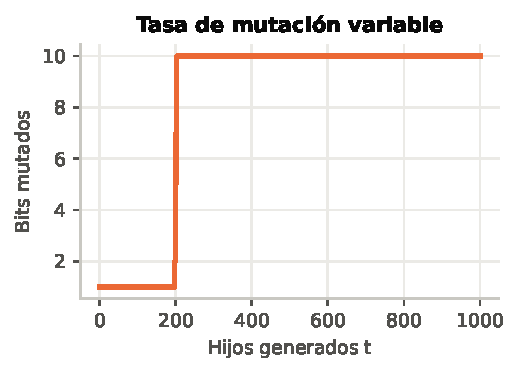
\includegraphics[width=0.48\textwidth]{fig_mutacion.pdf}
\caption{Número de bits mutados en función de los hijos generados ($m_f=10$, $m_c=200$, $m_g=2$).}
\label{fig:mut}
\end{figure}

\subsection{Reemplazo y criterio de parada}
El AG es de \textbf{estado estacionario}: en cada iteración se genera un solo hijo, que (i) se
descarta si ya existe un individuo idéntico en la población, para evitar la pérdida de diversidad,
o (ii) reemplaza a un individuo elegido al azar entre los que tienen costo mayor que el promedio.
Así el mejor individuo nunca se pierde (elitismo implícito).

El algoritmo se detiene cuando ocurre lo primero de:
\begin{enumerate}[nosep]
  \item se generan $T_{\max}$ hijos;
  \item pasan $T_{\text{sin mejora}}$ hijos sin mejorar la mejor solución (estancamiento);
  \item se supera un tiempo máximo.
\end{enumerate}
El Algoritmo~\ref{alg:ga} resume el procedimiento y la Tabla~\ref{tab:param} los parámetros.

\begin{algorithm}[H]
\caption{Algoritmo genético para el SCP}\label{alg:ga}
\begin{algorithmic}[1]
\State Generar $N$ individuos aleatorios y repararlos; evaluar su costo
\State $t\gets 0$
\While{no se cumpla el criterio de parada}
   \State $t\gets t+1$
   \State Seleccionar $P_1, P_2$ por torneo binario
   \State $H\gets$ CruceFusión$(P_1,P_2)$; \; $H\gets$ Mutar$(H,k(t))$; \; $H\gets$ Reparar$(H)$
   \If{$H$ no está duplicado en la población}
      \State Reemplazar un individuo al azar con costo mayor al promedio por $H$
      \State Actualizar la mejor solución si $f(H)$ es menor
   \EndIf
\EndWhile
\State \Return la mejor solución encontrada
\end{algorithmic}
\end{algorithm}

\begin{table}[H]
\centering\small
\caption{Parámetros del algoritmo genético.}\label{tab:param}
\begin{tabularx}{\textwidth}{l c X}
\toprule
Parámetro & Valor & Justificación \\
\midrule
Tamaño de población $N$ & 100 & Valor usado por \citet{beasley1996ga}; equilibra diversidad y costo por generación (ver Sección~\ref{sec:e3}). \\
Máximo de hijos $T_{\max}$ & 50\,000 & Límite superior de esfuerzo; en la práctica se activa antes el estancamiento. \\
Hijos sin mejora $T_{\text{sin mejora}}$ & 15\,000 & 150 veces el tamaño de la población sin progreso indica convergencia. \\
Tiempo máximo & 120 s & Salvaguarda para instancias grandes (60 s en el experimento de escalabilidad). \\
$m_f$, $m_c$, $m_g$ & 10, 200, 2 & Parámetros de la mutación variable de \citet{beasley1996ga}. \\
Selección & torneo binario & Presión selectiva moderada. \\
Semillas & 1 a 10 & 10 corridas independientes por instancia para medir la variabilidad. \\
\bottomrule
\end{tabularx}
\end{table}

% ==================================================================
\section{Detalles de implementación}
% ==================================================================
Todo el proyecto está en Python~3 con \texttt{numpy}, \texttt{pandas}, \texttt{PuLP}~2.9 (CBC),
\texttt{matplotlib} y \texttt{streamlit}. La estructura es:
\begin{itemize}[nosep]
  \item \texttt{src/instancia.py}: lectura del formato OR-Library, generación de instancias aleatorias y
  verificación de factibilidad.
  \item \texttt{src/exacto.py}: modelo PLEB con PuLP + CBC.
  \item \texttt{src/ga.py}: algoritmo genético (clase \texttt{AlgoritmoGenetico}) y la heurística voraz de
  Chvátal, usada solo como referencia.
  \item \texttt{src/experimentos.py}, \texttt{src/figuras.py}, \texttt{src/tablas.py}: experimentos, figuras y
  tablas de este informe.
  \item \texttt{app.py}: interfaz visual.
\end{itemize}

Para que el AG sea eficiente, la matriz $A$ se guarda como un arreglo booleano de \texttt{numpy} y,
además, para cada fila la lista de columnas que la cubren y para cada columna la lista de filas que
cubre. La reparación mantiene un vector de cobertura $w$ que se actualiza de forma incremental, sin
recalcular $A\mathbf{x}$ cada vez. Las corridas son reproducibles porque cada una usa un generador
\texttt{numpy.random.default\_rng(semilla)}.

\paragraph{Interfaz visual.} La aplicación de Streamlit (\texttt{streamlit run app.py}) tiene cinco
pestañas:
\begin{enumerate}[nosep]
  \item \emph{Instancia}: tamaño, densidad, distribución de costos y el modelo matemático.
  \item \emph{Método exacto}: costo, columnas seleccionadas, tiempo y estado.
  \item \emph{Algoritmo genético}: parámetros editables, curva de convergencia en vivo con la línea del
  óptimo y detalle por corrida.
  \item \emph{Comparación}: gap, tiempos y gráficos de barras de los tres métodos, coincidencia de
  columnas y descarga de las soluciones en CSV.
  \item \emph{Experimentos}: tablas y figuras de este informe.
\end{enumerate}
Permite usar instancias de la OR-Library, generar instancias aleatorias o subir un archivo propio.

% ==================================================================
\section{Experimentos computacionales}
% ==================================================================
\subsection{Instancias y protocolo}
Se usaron las 18 instancias disponibles de los conjuntos 4 (\texttt{scp41}--\texttt{scp49},
$200\times1000$) y 5 (\texttt{scp51}--\texttt{scp59}, $200\times2000$) de la
OR-Library~\citep{beasley1990orlib}, que provienen de \citet{balas1980}. Tienen densidad cercana
al 2\% y costos enteros entre 1 y 100. Se usan ampliamente como banco de pruebas y su óptimo es
conocido~\citep{beasley1996ga}. Para estudiar la escalabilidad se generaron instancias aleatorias de
$200\times2000$ a $1000\times10\,000$ con la misma densidad y rango de costos.

La calidad del AG se mide con el \emph{gap} relativo al valor del método exacto:
\[
\text{gap (\%)}=100\cdot\frac{f_{\text{AG}}-Z^\ast}{Z^\ast}.
\]
El AG se ejecutó 10 veces por instancia (semillas 1 a 10). Todas las pruebas se corrieron en un
procesador Intel Xeon de 2,1~GHz (2 núcleos virtuales, Linux, Python~3.13), sin paralelismo. Los
tiempos absolutos variarán en otro equipo, pero las tendencias se mantienen.

\subsection{E1: instancias OR-Library}
La Tabla~\ref{tab:e1} resume los resultados. El método exacto obtuvo en todas las instancias el valor
óptimo reportado en la literatura y probó su optimalidad, con un tiempo promedio de 0,09~s. El AG
alcanzó el óptimo en 15 de 18 instancias en al menos una corrida y en 77 de las 180 corridas
(43\%). Su gap promedio fue de 0,58\%, y el peor gap promedio por instancia fue de 1,90\%
(\texttt{scp49}). Las únicas instancias en que no llegó al óptimo en ninguna corrida fueron
\texttt{scp49}, \texttt{scp52} y \texttt{scp53}, con un mejor gap de 0,47\%, 0,99\% y 0,88\%. La
heurística voraz quedó en promedio a 4,3\% del óptimo, de modo que el AG mejora claramente la
solución constructiva.

\begin{table}[H]
\centering\scriptsize
\setlength{\tabcolsep}{3.5pt}
\caption{Resultados en las instancias OR-Library. $Z^\ast$: óptimo del método exacto; Greedy: costo
(gap \%); AG: mejor, promedio y peor costo en 10 corridas, gap promedio (\%), tiempo promedio (s) y
corridas que alcanzan el óptimo.}\label{tab:e1}
\begin{tabular}{l c r r r r r r r r c}
\toprule
& & \multicolumn{2}{c}{Exacto (CBC)} & \multicolumn{1}{c}{Greedy} & \multicolumn{6}{c}{Algoritmo genético} \\
\cmidrule(lr){3-4}\cmidrule(lr){5-5}\cmidrule(lr){6-11}
Instancia & $m\times n$ & $Z^\ast$ & t (s) & costo (gap) & mejor & prom. & peor & gap \% & t (s) & éxitos \\
\midrule
scp41 & 200$\times$1000 & 429 & 0,04 & 434 (1,2) & 429 & 431,4 & 433 & 0,56 & 2,91 & 1/10 \\
scp42 & 200$\times$1000 & 512 & 0,03 & 529 (3,3) & 512 & 513,6 & 525 & 0,31 & 2,85 & 8/10 \\
scp43 & 200$\times$1000 & 516 & 0,04 & 537 (4,1) & 516 & 516,0 & 516 & 0,00 & 3,11 & 10/10 \\
scp44 & 200$\times$1000 & 494 & 0,03 & 506 (2,4) & 494 & 496,4 & 502 & 0,49 & 3,09 & 7/10 \\
scp45 & 200$\times$1000 & 512 & 0,04 & 518 (1,2) & 512 & 512,4 & 514 & 0,08 & 3,32 & 8/10 \\
scp46 & 200$\times$1000 & 560 & 0,08 & 594 (6,1) & 560 & 560,9 & 561 & 0,16 & 3,07 & 1/10 \\
scp47 & 200$\times$1000 & 430 & 0,04 & 447 (4,0) & 430 & 430,6 & 434 & 0,14 & 3,67 & 7/10 \\
scp48 & 200$\times$1000 & 492 & 0,08 & 525 (6,7) & 492 & 492,7 & 493 & 0,14 & 2,73 & 3/10 \\
scp49 & 200$\times$1000 & 641 & 0,07 & 665 (3,7) & 644 & 653,2 & 661 & 1,90 & 3,40 & 0/10 \\
scp51 & 200$\times$2000 & 253 & 0,16 & 269 (6,3) & 253 & 256,8 & 266 & 1,50 & 3,88 & 5/10 \\
scp52 & 200$\times$2000 & 302 & 0,20 & 330 (9,3) & 305 & 307,0 & 313 & 1,66 & 4,22 & 0/10 \\
scp53 & 200$\times$2000 & 226 & 0,07 & 232 (2,7) & 228 & 228,2 & 229 & 0,97 & 3,31 & 0/10 \\
scp54 & 200$\times$2000 & 242 & 0,18 & 250 (3,3) & 242 & 242,7 & 243 & 0,29 & 3,45 & 3/10 \\
scp55 & 200$\times$2000 & 211 & 0,07 & 212 (0,5) & 211 & 211,1 & 212 & 0,05 & 3,78 & 9/10 \\
scp56 & 200$\times$2000 & 213 & 0,10 & 225 (5,6) & 213 & 213,9 & 218 & 0,42 & 2,83 & 7/10 \\
scp57 & 200$\times$2000 & 293 & 0,16 & 306 (4,4) & 293 & 295,5 & 298 & 0,85 & 3,56 & 1/10 \\
scp58 & 200$\times$2000 & 288 & 0,18 & 311 (8,0) & 288 & 290,1 & 302 & 0,73 & 3,48 & 2/10 \\
scp59 & 200$\times$2000 & 279 & 0,06 & 292 (4,7) & 279 & 279,6 & 281 & 0,22 & 3,28 & 5/10 \\
\midrule
\textbf{Promedio} & & & 0,09 & (4,3) & & & & 0,58 & 3,33 & 77/180 \\
\bottomrule
\end{tabular}
\end{table}

La Figura~\ref{fig:gap} muestra el gap por instancia: los puntos son el gap promedio del AG, las
barras verticales el rango de las 10 corridas y los rombos la heurística voraz. La
Figura~\ref{fig:tiempos} compara los tiempos en escala logarítmica. En estas instancias el AG tarda entre 19 y 104 veces más que CBC (mediana 51), pero encuentra su mejor solución en promedio a los 0,96~s. El resto del
tiempo lo dedica a confirmar el estancamiento.

\begin{figure}[H]
\centering
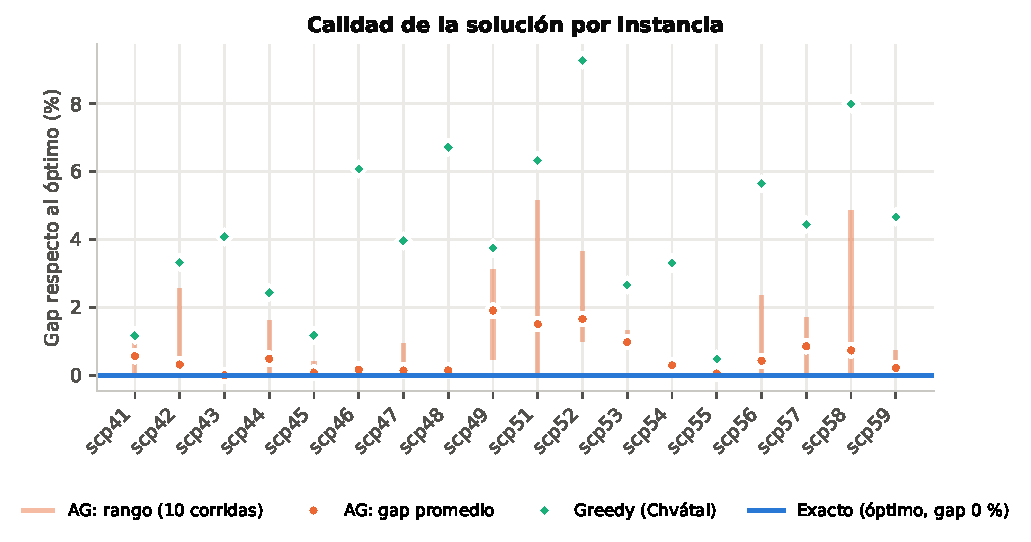
\includegraphics[width=\textwidth]{fig_gap_instancias.pdf}
\caption{Gap respecto al óptimo en cada instancia de la OR-Library.}\label{fig:gap}
\end{figure}

\begin{figure}[H]
\centering
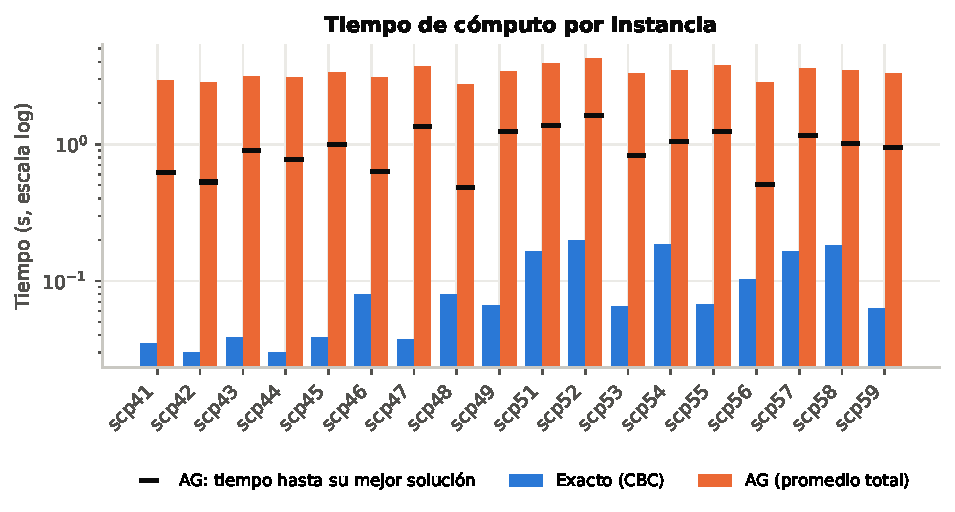
\includegraphics[width=\textwidth]{fig_tiempos_instancias.pdf}
\caption{Tiempo de cómputo del método exacto y del AG (escala logarítmica). La marca negra indica
el tiempo promedio en que el AG encontró su mejor solución.}\label{fig:tiempos}
\end{figure}

\paragraph{Comportamiento del AG.} La Figura~\ref{fig:conv} muestra la convergencia en
\texttt{scp41} (fácil) y \texttt{scp49} (la más difícil para el AG). El costo del mejor individuo cae
bruscamente durante los primeros 500--1000 hijos y luego mejora a pasos cada vez más espaciados. El
costo promedio de la población, en gris, se acerca al del mejor, lo que indica que la población
converge. Este hecho se confirma con los hijos duplicados: en promedio, 11\,185 de los 20\,037 hijos
generados por corrida (56\%) fueron copias de individuos existentes y se descartaron. En todas las
corridas el criterio que detuvo el algoritmo fue el estancamiento. En \texttt{scp49} las corridas
quedan atrapadas en óptimos locales distintos (entre 644 y 661), lo que explica la mayor
variabilidad (desviación estándar de 5,3).

\begin{figure}[H]
\centering
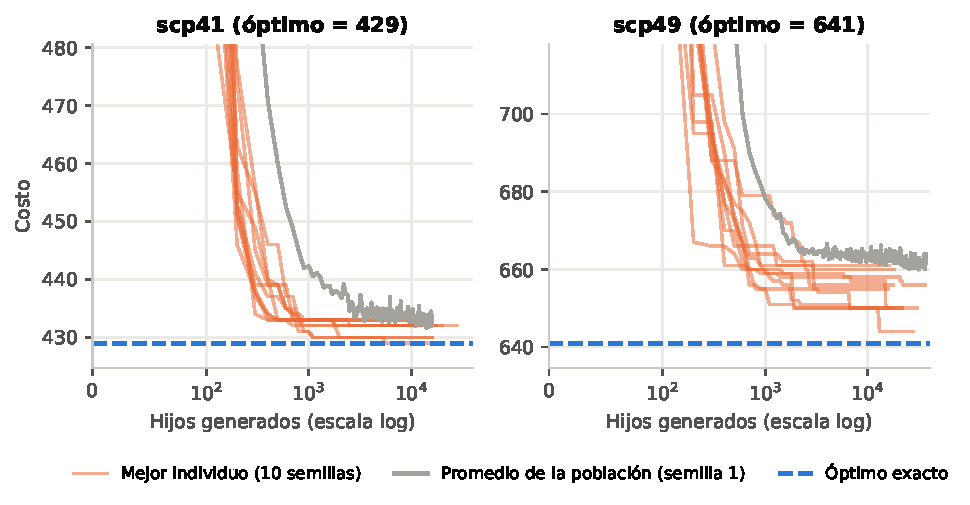
\includegraphics[width=\textwidth]{fig_convergencia.pdf}
\caption{Convergencia del AG: mejor individuo de las 10 corridas y promedio de la población
(semilla 1). La línea azul punteada es el óptimo del método exacto.}\label{fig:conv}
\end{figure}

\subsection{E2: escalabilidad}
La Tabla~\ref{tab:e2} y la Figura~\ref{fig:esc} muestran lo que ocurre al aumentar el tamaño, con un
límite de 180~s para CBC y de 60~s para el AG (3 corridas). El tiempo del método exacto crece de forma
exponencial: pasa de 0,06~s ($200\times2000$) a 121~s ($600\times6000$), y en las dos instancias
más grandes alcanza el límite sin poder probar la optimalidad. El tiempo del AG crece de forma casi
lineal, de 4,8 a 13,6~s. En las instancias en que CBC terminó, el AG quedó entre 0,9 y 2,2\% del
óptimo. En $800\times8000$ la mejor corrida del AG (166) superó la solución de CBC (167), y en
$1000\times10\,000$ incluso el \emph{promedio} del AG (183) fue mejor que CBC (184). El gap negativo
significa que la metaheurística encontró una solución mejor que la que el solver exacto logró en
el tiempo disponible, usando menos del 8\% de ese tiempo.

\begin{table}[H]
\centering\small
\caption{Escalabilidad en instancias aleatorias (densidad 2\%). El gap de las dos últimas filas se
calcula respecto a la mejor solución de CBC, no respecto a un óptimo probado.}\label{tab:e2}
\begin{tabular}{c r l r r r r r}
\toprule
& \multicolumn{3}{c}{Exacto (CBC)} & \multicolumn{4}{c}{AG (3 corridas)}\\
\cmidrule(lr){2-4}\cmidrule(lr){5-8}
$m\times n$ & costo & estado & t (s) & mejor & prom. & t (s) & gap \% \\
\midrule
200$\times$2000 & 229 & Óptimo probado & 0,06 & 229 & 231,00 & 4,77 & 0,87 \\
400$\times$4000 & 235 & Óptimo probado & 4,28 & 239 & 239,67 & 7,40 & 1,99 \\
600$\times$6000 & 196 & Óptimo probado & 121,23 & 200 & 200,33 & 10,85 & 2,21 \\
800$\times$8000 & 167 & Límite 180 s & 180,54 & 166 & 167,67 & 11,63 & 0,40 \\
1000$\times$10000 & 184 & Límite 180 s & 180,78 & 182 & 183,00 & 13,56 & $-$0,54 \\
\bottomrule
\end{tabular}
\end{table}

\begin{figure}[H]
\centering
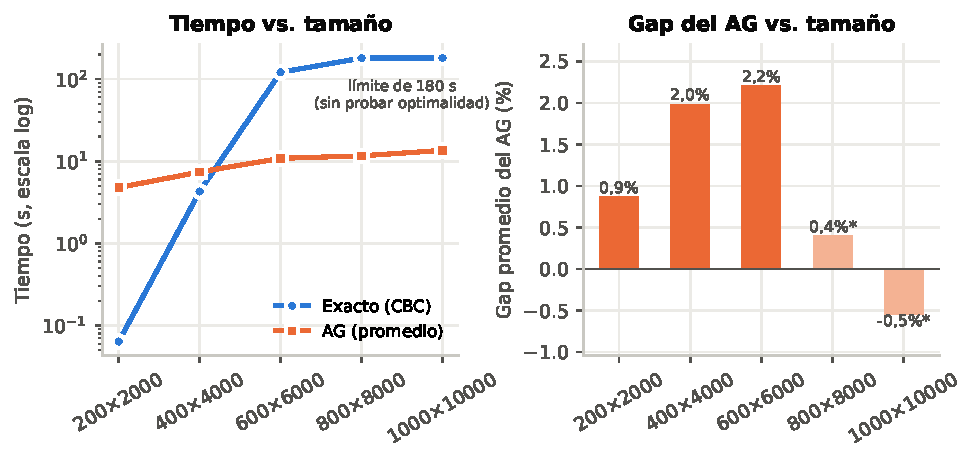
\includegraphics[width=\textwidth]{fig_escalabilidad.pdf}
\caption{Tiempo (escala log) y gap promedio del AG según el tamaño. Las barras claras (*) se
comparan con la mejor solución de CBC al límite de tiempo.}\label{fig:esc}
\end{figure}

\subsection{E3: sensibilidad de parámetros}\label{sec:e3}
Para justificar los parámetros se probaron $N\in\{50,100,200\}$ y $m_f\in\{5,10,20\}$ en
\texttt{scp49} y \texttt{scp57}, con 5 semillas por combinación (Tabla~\ref{tab:e3} y
Figura~\ref{fig:sens}).
En promedio sobre ambas instancias, una población más grande reduce ligeramente el gap: 1,46\% con
$N=50$, 1,18\% con $N=100$ y 1,06\% con $N=200$. El tiempo no aumenta (4,4, 4,1 y 4,0~s), porque
el criterio de estancamiento se activa en un número similar de hijos. Una mutación final más fuerte
también reduce el gap (1,49\%, 1,20\% y 1,01\% para $m_f=5$, 10 y 20), pero sí aumenta el
tiempo (3,4, 3,9 y 5,1~s): más diversidad prolonga la búsqueda antes de estancarse. Las diferencias
son pequeñas comparadas con la variación entre semillas, y la mejor combinación cambia de una
instancia a otra (por ejemplo, $N=50$, $m_f=10$ en \texttt{scp49} y $N=100$, $m_f=20$ en
\texttt{scp57}). Por eso se mantuvo la configuración de referencia de \citet{beasley1996ga}
($N=100$, $m_f=10$), que ofrece un buen equilibrio entre calidad y tiempo. Las configuraciones con
$N=200$ o $m_f=20$ son una alternativa razonable si se dispone de más tiempo.

\begin{table}[H]
\centering\small
\caption{Gap promedio (\%) y tiempo promedio (s) según el tamaño de población $N$ y $m_f$ (5 semillas).}\label{tab:e3}
\begin{tabular}{c c r r r r}
\toprule
& & \multicolumn{2}{c}{\texttt{scp49}} & \multicolumn{2}{c}{\texttt{scp57}} \\
\cmidrule(lr){3-4}\cmidrule(lr){5-6}
$N$ & $m_f$ & gap \% & t (s) & gap \% & t (s) \\
\midrule
50 & 5 & 2,50 & 3,39 & 1,43 & 4,17 \\
50 & 10 & 0,75 & 5,20 & 1,91 & 4,01 \\
50 & 20 & 1,03 & 4,33 & 1,16 & 5,19 \\
100 & 5 & 1,40 & 3,03 & 1,43 & 2,97 \\
100 & 10 & 1,78 & 3,77 & 0,89 & 3,43 \\
100 & 20 & 1,09 & 6,23 & 0,48 & 5,23 \\
200 & 5 & 1,65 & 3,42 & 0,55 & 3,45 \\
200 & 10 & 1,34 & 3,83 & 0,55 & 3,31 \\
200 & 20 & 1,47 & 4,77 & 0,82 & 4,91 \\
\bottomrule
\end{tabular}
\end{table}

\begin{figure}[H]
\centering
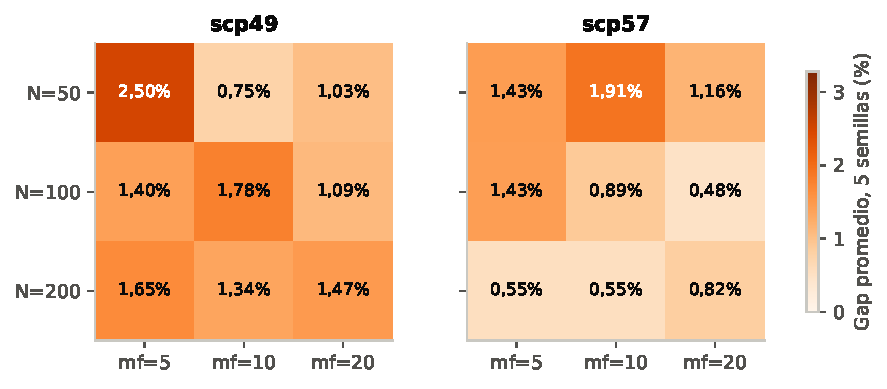
\includegraphics[width=\textwidth]{fig_sensibilidad.pdf}
\caption{Gap promedio del AG según el tamaño de población y el parámetro $m_f$ de la mutación.}\label{fig:sens}
\end{figure}

% ==================================================================
\section{Comparación y discusión}
% ==================================================================
\paragraph{Calidad de la solución.} El método exacto siempre entrega la solución óptima, con
certificado de optimalidad, cuando termina. El AG no da esa garantía: en las instancias de la
OR-Library alcanzó el óptimo en 15 de 18 instancias. En las demás quedó a menos de 1\% en su
mejor corrida y a menos de 2\% en promedio. Su resultado depende de la semilla, por lo que conviene
ejecutarlo varias veces.

\paragraph{Tiempo de cómputo.} En instancias pequeñas y medianas CBC es mucho más rápido, porque la
relajación lineal del SCP con costos da cotas muy ajustadas y los planos de corte cierran la brecha
casi sin ramificar. Cuando el tamaño crece, el número de nodos del árbol aumenta de forma
exponencial y el tiempo se dispara. El tiempo del AG depende del número de hijos y del costo de la
reparación, que crece aproximadamente en proporción al tamaño de la matriz. Por eso el punto de
cruce aparece entre $400\times4000$ y $600\times6000$.

\paragraph{¿Obtuvo el AG la solución óptima?} Sí, en 15 de las 18 instancias de la OR-Library, con
el 43\% de las corridas exitosas. En \texttt{scp49}, \texttt{scp52} y \texttt{scp53} quedó a 3, 3 y
2 unidades del óptimo en su mejor corrida (gaps de 0,47\%, 0,99\% y 0,88\%). En las
instancias grandes, donde el óptimo no se pudo probar, el AG igualó o mejoró la mejor solución
conocida.

\begin{table}[H]
\centering\small
\caption{Ventajas y desventajas de cada enfoque.}\label{tab:vd}
\begin{tabularx}{\textwidth}{l X X}
\toprule
& Método exacto (PLEB + CBC) & Algoritmo genético \\
\midrule
Ventajas &
Garantiza y certifica el óptimo; determinista y reproducible; fácil de modelar con un solver; muy rápido en instancias pequeñas y medianas. &
Tiempo controlable y casi lineal en el tamaño; entrega buenas soluciones en todo momento; escala a instancias grandes; se adapta fácilmente a variantes del problema. \\
\addlinespace
Desventajas &
Tiempo exponencial en el peor caso; en instancias grandes puede no terminar y solo entregar una solución factible; necesita un solver y bastante memoria. &
No garantiza el óptimo ni indica qué tan lejos está; resultados variables según la semilla; requiere ajustar parámetros; tiende a converger prematuramente (56\% de hijos duplicados). \\
\bottomrule
\end{tabularx}
\end{table}

% ==================================================================
\section{Conclusiones}
% ==================================================================
\begin{itemize}
  \item El SCP se formuló como un modelo de programación lineal entera binaria con $n$ variables y
  $m$ restricciones de cobertura. Resuelto con PuLP y CBC, obtuvo el óptimo de las 18 instancias de
  la OR-Library en menos de 0,2~s cada una, lo que valida el modelo y la lectura de los datos.
  \item El algoritmo genético, con reparación especializada, cruce por fusión y mutación variable,
  encontró el óptimo en 15 de 18 instancias, con un gap promedio de 0,58\% y siempre mejor que la
  heurística voraz (4,3\%).
  \item No hay un método mejor en todos los casos. Para instancias del tamaño de la OR-Library el
  método exacto es preferible: es más rápido y certifica el óptimo. A medida que el problema crece,
  el método exacto se vuelve muy costoso, y el AG ofrece soluciones de igual o mejor calidad en una
  fracción del tiempo.
  \item El principal punto débil del AG es la convergencia prematura. Como trabajo futuro se propone
  agregar búsqueda local a la mejor solución (un algoritmo memético), reiniciar parte de la población
  al detectar estancamiento, o combinar ambos enfoques: usar la solución del AG como solución inicial
  del solver exacto.
\end{itemize}

\bibliographystyle{plainnat}
\bibliography{referencias}

\end{document}
